\documentclass{easychair}

% \usepackage{doc}
\usepackage{setspace}
\usepackage{verbatim}
\usepackage{amssymb}
\usepackage{wasysym}
\usepackage[straightquotes]{newtxtt}


%----Making things more compact
%----Suppress extra space in texttt mode
%\AddToHook{cmd/ttfamily/after}{\frenchspacing}
% \newcommand{\smalltt}[1]{\small \texttt{#1}}

\newenvironment{packed_itemize}{
\vspace*{-0.3em}
\begin{itemize}
\setlength{\partopsep}{0pt}
\setlength{\itemsep}{1pt}
\setlength{\parskip}{0pt}
\setlength{\parsep}{0pt}
}{\end{itemize}}
\newenvironment{packed_enumerate}{
\vspace*{-0.3em}
\begin{enumerate}
\setlength{\partopsep}{0pt}
\setlength{\itemsep}{1pt}
\setlength{\parskip}{0pt}
\setlength{\parsep}{0pt}
}{\end{enumerate}}
% \renewcommand{\textfraction}{0.07}
% \renewcommand{\topfraction}{0.9}
% \renewcommand{\bottomfraction}{0.9}
% \renewcommand{\floatpagefraction}{0.66}
% \setlength{\floatsep}{2.0pt plus 2.0pt minus 2.0pt}
% \setlength{\textfloatsep}{5.0pt plus 2.0pt minus 0.0pt}

\newcommand{\dav}[1]{{\color{red}{David: {#1}}}}
\newcommand{\jack}[1]{{\color{red}{Jack: {#1}}}}

\title{Towards StarExec in the Cloud}

\author{
  David Fuenmayor\inst{1}
\and
  Jack McKeown\inst{2}
\and
  Geoff Sutcliffe\inst{2}
}

\institute{
  University of Bamberg,
  Bamberg, Germany\\
  \email{david.fuenmayor@uni-bamberg.de}
\and
  University of Miami,
  Miami, USA\\
  \email{jam771@miami.edu,geoff@cs.miami.edu}
}

\authorrunning{Fuenmayor, McKeown, Sutcliffe}
\titlerunning{Stars in the Clouds}

\begin{document}
\maketitle

%--------------------------------------------------------------------------------------------------
\begin{abstract}
StarExec has been central to much progress in logic solvers over the last 10 years.
It was recently announced that StarExec Iowa will be decommissioned, and while StarExec Miami 
will continue to operate while funding is available, it will not be able to support all the 
logic solver communities currently using the larger StarExec Iowa. 
In the long term StarExec will necessarily have to migrate to new compute environments.
This paper describes work being done to reengineer StarExec as a cloud-native application using
container technology and infrastructure-as-code practices.
The first step has been to containerise StarExec and ATP systems so that they can be run on a 
broad range of computer platforms. 
The next step in process is to write a new backend in StarExec so that Kubernetes can be used to 
orchestrate distribution of StarExec job pairs over whatever compute nodes are available.
Supported by an Amazon Research Award, a new version of StarExec will be deployed in AWS.
\end{abstract}
%--------------------------------------------------------------------------------------------------
% Geoff
\section{Introduction}
\label{Introduction}

Automated Theorem Proving (ATP) is concerned with the development and use of tools that automate 
sound reasoning: the derivation of conclusions that follow inevitably from facts.
Automated Theorem Proving (ATP) is at the heart of many computational tasks, in particular for
verification \cite{Har06,HH19} and security \cite{Coo18}.\footnote{%
In AWS -
\href{https://aws.amazon.com/what-is/automated-reasoning/}{\tt aws.amazon.com/what-is/automated-reasoning/}, 
\href{https://aws.amazon.com/security/provable-security//}{\tt aws.amazon.com/security/provable-security/}.} 
New and emerging application areas include
chemistry \cite{Yad17}, 
biology \cite{CC+13}, 
medicine \cite{HLB05},
elections \cite{Nip09,BDS17}, 
auctions \cite{CK+15}, 
privacy \cite{Lib20},
law \cite{PS15}, 
ethics \cite{DF+16}, 
religion \cite{OZ11,BW14-ECAI,Hor19},
and business \cite{Han98}.
ATP systems are also used as components of more complex Artificial Intelligence (AI) systems,
and the impact of ATP is thus extended into many facets of society.
% in areas such as 
% knowledge representation \cite{TR+04}, 
% natural language processing \cite{BM05}, 
% planning \cite{NV07}, 
% agents \cite{TBP03}, 
% commonsense reasoning \cite{MS05}, 
% and the semantic web \cite{McG04}.

The Thousands of Problems for Theorem Provers (TPTP) World \cite{Sut24} is a well established 
infrastructure that supports research, development, and deployment of ATP systems.
The TPTP World includes 
the TPTP problem library \cite{Sut17},
the TSTP solution library \cite{Sut10},
standards for writing ATP problems and reporting ATP solutions \cite{SS+06,Sut08-KEAPPA},
tools and services for processing ATP problems and solutions \cite{Sut10},
and it supports the annual CADE ATP System Competition (CASC)~\cite{Sut16}.
Since its first release in 1993 the ATP community has used the TPTP World as an appropriate and 
convenient infrastructure for ATP system development, evaluation, and application.
The TPTP World has a diverse, engaged, and sustained user community, with various parts of the 
TPTP World being deployed in a range of applications in both academia and industry.\footnote{%
TPTP has contributed to recognized research in 627 publications that cite \cite{Sut17},
according to Google Scholar.}
The web page \href{https://www.tptp.org}{\tt www.tptp.org} provides access to all components.

The TPTP problem library was motivated by the need to provide support for meaningful ATP system 
evaluation.
The need to provide support for meaningful system evaluation has been recognized in many other 
logic solver communities, e.g., TPTP~\cite{SS01}, SAT~\cite{HS00-SATLIB}, SMT~\cite{CSW15},
Termination~\cite{MZ07}, etc.
For many years testing of logic solvers was done on individual developers' computers. 
In 2010 a proposal for centralised hardware and software support was submitted to the NSF,
and in 2011 a \$2.11 million grant\footnote{%
NSF Awards 1058748 and 1058925, led by Aaron Stump and Cesare Tinelli at the University of Iowa} 
was awarded.
This grant led to the development and availability of StarExec Iowa~\cite{SST14} in 2012,
and a subsequent \$1.00 million grant\footnote{%
NSF Award 1730419} in 2017 expanded StarExec to Miami.
StarExec has been central to much progress in logic solvers over the last 10 years, supporting
16 logic solver communities, used for running many annual competitions~\cite{BB+19}, and 
supporting many many users.
StarExec Iowa provides community infrastructure for many logic solver communities,
e.g., ASP, QBF, SAT, SMT, Termination, etc, while StarExec Miami is used by the TPTP community.
StarExec Miami has features that take advantage of TPTP standards, and is also used to host CASC.

It was recently announced that StarExec Iowa will be decommissioned. 
The maintainer of StarExec Iowa explained that ``the plan is to operate StarExec as usual for 
competitions Summer 2024 and Summer 2025, and then put the system into a read-only mode for one 
year (Summer 2025 to Summer 2026)''.
The 2017 grant for StarExec Miami paid for the hardware and three years of system administration.
The hardware is still hosted by the University of Miami High Performance Computing group,
funded on a shoe-string budget by the TPTP World.
While StarExec Miami will continue to operate while funding is available, it will not be able
to support all the logic solver communities currently using the larger StarExec Iowa.
In the long term StarExec will necessarily have to migrate to new compute environments, and 
several plans are (at the time of writing) being discussed.
This paper describes work being done to reengineer StarExec as a cloud-native application using
container technology and infrastructure-as-code practices.
The first step has been to containerise\footnote{%
Strictly, ``images'' are built, and the images are deployed in containers. 
But keeping with common use of the terminology, we say ``container images'' and ``containerise''.} 
StarExec and ATP systems so that they can be run on a broad range of computer platforms.
The next step in process is to write a new backend in StarExec so that Kubernetes can be used to
orchestrate distribution of StarExec job pairs over whatever compute nodes are available.
Supported by an Amazon Research Award (see Section~\ref{StarExecK}) a new version of StarExec
will be deployed in AWS.
This StarExec instance will be fully functional and available to the community (as much as our 
budget allows). 
It will also serve as an exemplary implementation for those willing to deploy their own, possibly 
customized, StarExec on their own computers or in the cloud.

\paragraph{This paper is organized as follows:}
Section~\ref{Background} provides a short background to ATP systems, StarExec, and 
containerisation.
Section~\ref{ContainerisingStarExec} describes how StarExec has been containerised, and
Section~\ref{ContainerisingATPSystems} describes how ATP systems have been containerised.
Section~\ref{StarExecK} explains how the containerised StarExec and ATP systems will be deployed 
in a Kubernetes setting.
Section~\ref{Conclusion} concludes and looks forward to future work.

\vspace*{1em}
\noindent
All the software described in the paper is available from~\ldots \\
\hspace*{1cm}\href{https://github.com/StarExecMiami/StarExec-ARC}{\tt github.com/StarExecMiami/StarExec-ARC}.

%--------------------------------------------------------------------------------------------------
\section{Background}
\label{Background}

%--------------------------------------------------------------------------------------------------
\subsection{StarExec}
\label{StarExec}

Figure~\ref{ArchitectureS} shows the architecture of the currently deployed StarExec Miami.
The hardware consists of a single head node and multiple compute nodes.
The head node provides the browser interface for users, in particular it accepts job requests
that generate job pairs consisting of an ATP system and a problem file, does internal scheduling,
and uses the SUN Grid Engine (SGE) to distribute the job pairs to the compute nodes.
(For development and testing, the head node can also run job pairs itself using a local backend.)
The head node maintains a relational MariaDB database, and all the nodes access an NFS mounted
shared file system.
The database records everything, including locations of the ATP systems' files and the problem 
files in the file system. 
Job pairs executing on a compute node have their time and memory usage limited and reported
by the {\tt runsolver}~\cite{Rou11} utility (the {\tt BenchExec}~\cite{BLW19} utility in 
StarExec Iowa).
The results and resource usage data from completed job pairs are stored in the file system, 
and recorded in the database.
The browser interface provides the necessary facilities for user management, uploading ATP 
systems, uploading problem
files, browsing the ATP systems and problems, creating jobs, imposing resource limits in jobs,
tracking job progress, browsing and downloading job results, and deleting ATP systems, problems, 
jobs, etc.

\begin{figure}[htb]
\begin{center}
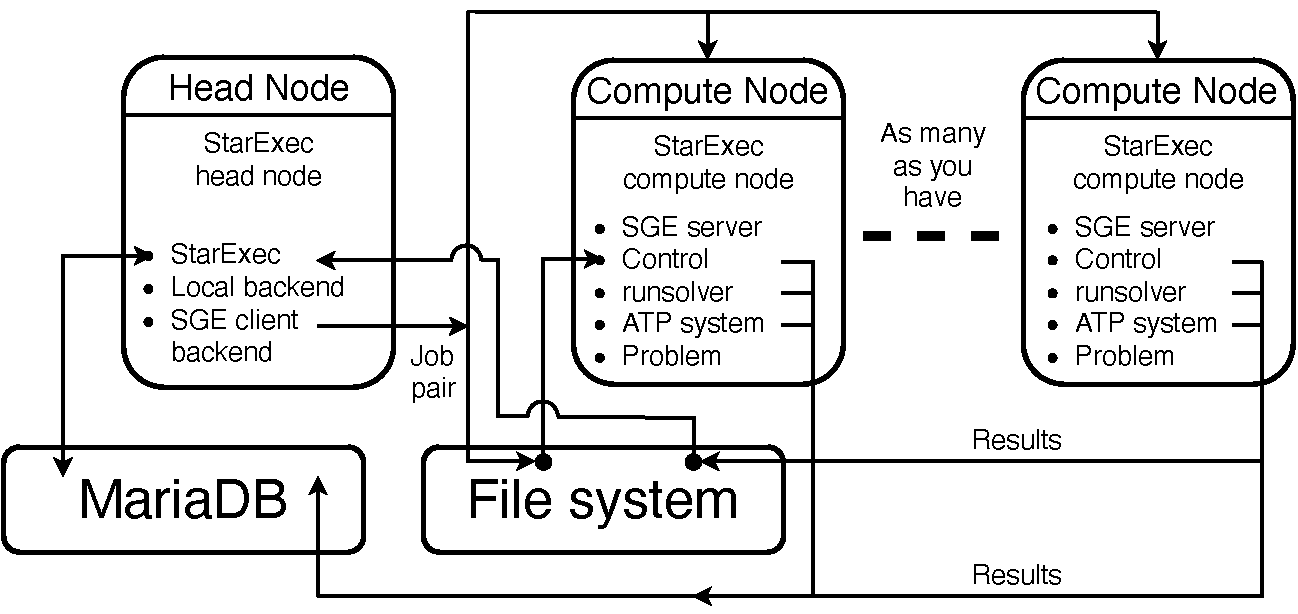
\includegraphics[width=0.8\textwidth]{ArchitectureS}
\caption{StarExec Architecture}
\label{ArchitectureS}
\end{center}
\end{figure}

%--------------------------------------------------------------------------------------------------
\subsection{ATP Systems}
\label{ATPSystems}

ATP Systems are complex pieces of software, typically using advanced data structures~\cite{Sch13}, 
sophisticated algorithms~\cite{Vor01}, and tricky code optimizations~\cite{Sch06}.
They are written in a variety of programming languages: Prolog~\cite{Ott23,Hol23}, 
Scala~\cite{SB18}, C~\cite{SCV19}, C++~\cite{RV02-AICOMM}, OCaml~\cite{Kor06}, Python~\cite{SP20}, 
etc.
Their build processes include techniques such as parser generators~\cite{Ste21}, Makefiles,
code repositories, specific versions of libraries, etc.
For a user who is focussed on an application of ATP,
% , e.g. (with a few exemplar references), in 
% mathematics \cite{Qua92-Book,MP96}, logic~\cite{GO86,Jec95}, management~\cite{PB+92-TR,PM94}, 
% planning \cite{SE94}, 
installing an ATP system can be a deal breaker. 
Many early users selected a weaker system, e.g., Otter~\cite{McC03-Otter}, for their experiments 
because it was readily available and easy enough to install.
% As the TPTP World evolved it was clear that more powerful ATP systems were available, especially
% evident in the CADE ATP System Competition (CASC)~\cite{Sut16}.
% However, these more powerful systems were often not as easy to obtain and install.
% This was a key motivation for the creation of the SystemOnTPTP service~\cite{Sut00-CADE-17}.
% SystemOnTPTP allows users to
% The ATP systems in SystemOnTPTP are installed by the third author, often with help from the
% individual system developers.
There have been some proposals for standardising the ATP system build process, e.g.,
\href{https://tptp.org/Proposals/SystemBuild.html}{\tt tptp.org/Proposals/SystemBuild.html}, 
but the diversity of ATP system software makes conformity nigh impossible.
An alternative is to push the task back on the system developers, and one approach to this is
containerising ATP systems, as discussed in Section~\ref{ContainerisingATPSystems}.

%--------------------------------------------------------------------------------------------------
\subsection{Containerisation}
\label{Containerisation}

Containers are a technology stemming from the concept of operating-system-level 
virtualization.\footnote{%
See \href{https://en.wikipedia.org/wiki/OS-level_virtualization}{\tt en.wikipedia.org/wiki/OS-level\_virtualization}}
In a nutshell, a container is a lightweight, isolated environment that packages and runs applications with all their dependencies as a self-contained unit in user space, while safely sharing the (Linux) kernel with other containers. This encapsulation facilitates seamless software deployment across diverse computing landscapes. 
Containers are specified using read-only templates, called ``images'', which contain all necessary components and instructions for creating a container, including application code, runtime platform, libraries, environment variables, and configuration files. The task of generating a container image for an existing application so it can be run as a container is often referred to as ``containerisation''.

Containerising an application offers numerous benefits, including scalability, resource efficiency, enhanced 
security, and improved observability. 
Since containers share the host operating system's kernel, they incur less overhead compared to 
traditional virtualisation techniques. 
This characteristic enables containers to be started and stopped quickly, facilitating rapid 
scaling of applications to meet fluctuating demands. 
Containerisation also supports observability akin to bare-metal environments through kernel-level 
mechanisms such as eBPF\footnote{%
Extended Berkeley Packet Filter, see \href{https://en.wikipedia.org/wiki/EBPF}{\tt en.wikipedia.org/wiki/EBPF}}
and cgroups\footnote{%
Linux's control groups, see \href{https://en.wikipedia.org/wiki/Cgroups}{\tt en.wikipedia.org/wiki/Cgroups}}, 
which enable sophisticated monitoring and resource management. 
The isolation provided by containers helps prevent conflicts between applications and enhances 
security by limiting the impact of potential vulnerabilities.

Popular containerisation platforms, e.g., Docker, Podman, LXD, and rkt, have significantly 
contributed to the widespread adoption of container technology within the modern IT landscape. 
Notably, Kubernetes (often abbreviated as K8s) has emerged as the de-facto industry standard for 
container orchestration: automating the deployment, scaling, and management of containerised 
applications. 
Kubernetes' YAML-based configuration manifests (JSON-variants are also supported) have become 
widely adopted as a language for  declarative infrastructure-as-code (IaC), enabling developers 
and operations teams to manage infrastructure through declarative, version-controlled code, 
rather than through the traditional error-prone mixture of imperative scripts and manual processes. 
IaC thus facilitates consistent, repeatable, and automated provisioning and deployment of servers, 
networks, and other infrastructure components.

As an ``operating system for the cloud'', Kubernetes offers several distributions with varying 
levels of functionality (and complexity). 
Nowadays, there exist several lightweight production-ready distributions, e.g., 
k3s (\href{https://k3s.io/}{\tt k3s.io}), k0s (\href{https://k0sproject.io/}{\tt k0sproject.io}), 
and microK8s (\href{https://microk8s.io/}{\tt microk8s.io}), that greatly simplify the deployment 
and management of Kubernetes environments, especially in development, testing, and small-scale 
production scenarios. 
These distributions provide an accessible entry point for organizations and individuals looking 
to adopt Kubernetes without the overhead of its full-scale versions, thus democratizing access 
to this pivotal technology.

%--------------------------------------------------------------------------------------------------
\section{Containerising StarExec}
\label{ContainerisingStarExec}

StarExec (see Section~\ref{StarExec}) is based around a head node that coordinates activities, 
in particular the creation of jobs as sets of job pairs, with each pair consisting of an ATP 
system and a problem file. 
MariaDB is used to store job information and results, and NFS is used to share disk space between 
the head node and compute nodes. 
StarExec currently offers two backends for running job pairs: the local backend that runs pairs on 
the same computer as the head node, and the Sun Grid Engine (SGE) backend that sends pairs out to 
compute nodes.

So far, the head node with a local backend has been successfully containerised - see the
{\tt starexec-containerised} directory of the GitHub repository.
It includes~\ldots
\begin{packed_itemize}
\item A {\tt Dockerfile} for building a StarExec image with a local backend.
\item A StarExec configuration file (database credentials, special StarExec directory paths, 
      default StarExec users, NFS mount path, etc.).
\item Various scripts used in the {\tt Dockerfile} to configure and build StarExec.
      These scripts are responsible for: 
      \begin{packed_itemize}
      \item Installing and configuring StarExec dependencies including Java, Apache Tomcat, ant, 
            MariaDB, SPSS, and more.
      \item Creating new user accounts (at the operating system level) used for running jobs.
      \item Changing permissions of certain files and directories that StarExec depends on.
      \item Building StarExec using ant, which also initializes the database.
      \end{packed_itemize}
\item A {\tt README.md} file explaining how to build and run the image.
\end{packed_itemize}

The deployment of StarExec Miami was a real challenge, requiring installation and configuration 
of many pieces of software.
The containerisation approach aims to make this process simple and repeatable, eliminating the 
need to understand the complex environment requirements of StarExec. 
While the containerisation of StarExec with a local backend is somewhat valuable on its own,
it is most importantly a first step towards the deployment of a full StarExec cluster in the cloud.
Section~\ref{StarExecK} explains how this will be done.

% \dav{A related idea is that, following the IaC approach, the resulting sources (shell scripts, config files, Dockerfiles, etc) can be made available (e.g. as a public Git repository) to a community of users/developers, so they can build, test (and run) their own (e.g. forked) StarExec(s). This also enables people to become contributors of other StarExec repos (e.g. Miami's) by sending pull requests or the like. I think this is a good means to promote the survival of StarExec as a decentralized open-source project.}

%--------------------------------------------------------------------------------------------------
\section{Containerising ATP Systems}
\label{ContainerisingATPSystems}

While the grand plan is to deploy ATP systems in a containerised StarExec, and in a Kubernetes 
hosted version of StarExec, containerising ATP systems is independently useful because it allows 
ATP systems to be easily deployed in users' applications.
It would be great if ATP systems developers become super enthusiastic about containerising their 
systems after reading this section~\smiley.

The ATP systems' are containerised in a hierarchy, shown in Figure~\ref{ImageDAG}.
The underlying operating system is {\tt ubuntu:latest} from {\tt dockerhub}~\ldots\\
\hspace*{1cm}\href{https://hub.docker.com/_/ubuntu}{\tt hub.docker.com/\_/ubuntu} \\
The {\tt ubuntu-arc}\footnote{%
``arc'' for ``Automated Reasoning Containerisation, or Automated Reasoning in the Cloud''.}
container image adds to {\tt ubuntu:latest} using {\tt apt-get} to 
install common software such as {\tt cmake}, {\tt git}, {\tt tcsh}, {\tt python3}, and {\tt wget}.
{\tt ubuntu-arc} also creates an {\tt artifacts} directory where the components required for 
an ATP system's execution are placed.

The {\tt tptp-world} container image provides utilities from the TPTP World that are used by 
ATP systems, e.g., {\tt SPCForProblem} detects the Specialist Problem Class (SPC) \cite{SS01} of 
a problem that is used by some ATP systems to decide on what search parameters to use.
To support these utilities some libraries that are not part of the {\tt ubuntu-arc} have
to be added.
Additionally, the {\tt runsolver} utility for limiting and reporting the resources used by an 
ATP system is added.
(See Section~\ref{RLR} for information about the forthcoming {\tt ResourceLimitRun} utility
that will replace {\tt runsolver}.)
The details of building the {\em ATP-system:version} and {\em ATP-system:version}{\tt -RLR}
container images are provided in Section~\ref{BuildingATPSystemImages}.

\begin{figure}[htb]
\begin{center}
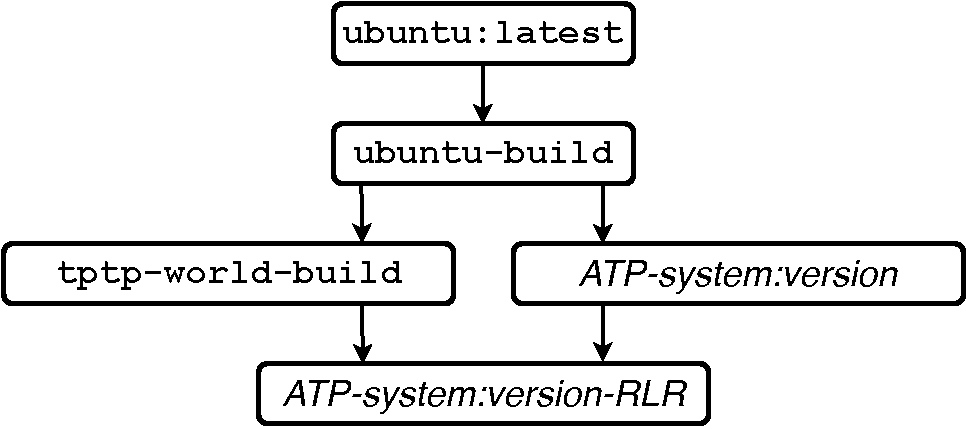
\includegraphics[width=0.8\textwidth]{ImageDAG} 
\caption{ATP System Container Image Hierarchy}
\label{ImageDAG}
\end{center}
\end{figure}

%--------------------------------------------------------------------------------------------------
\subsection{Building ATP System Containers}
\label{BuildingATPSystemImages}

Each {\em ATP-system:version} container image is built on top of the {\tt ubuntu-arc} container 
image, and with the {\tt tptp-world} container image forms the base for the final 
{\em ATP-system:version}{\tt -RLR} container image.
The {\em ATP-system} is the container name, and the {\em version}/{\em version}{\tt -RLR} are 
the container tags.
Podman\footnote{Our containerisation efforts are carried out using Podman, which is designed to work as a drop-in replacement for Docker (simply aliasing {\tt podman} to {\tt docker} is endorsed in the documentation).} requires the container name to be lowercase, so, e.g., E's container is named {\tt eprover}.
The ``{\tt RLR}'' refers to the ``Resource Limited Run'' program used to monitor and limit the 
resources used by the ATP system, either {\tt runsolver} or {\tt ResourceLimitRun}.
The files for containerising some ATP systems are in the {\tt provers-containerised} directory 
of the GitHub repository.
A {\tt Makefile} to containerise E, Leo-III, and Vampire is included.

Each {\em ATP-system:version} container image adds the ATP system's executables to 
{\tt ubuntu-arc}.
The ATP system is retrieved online, e.g., from a GitHub repository, and the necessary commands
to build the executables are run.
The executables are copied into the {\tt /artifacts} directory.
The choice of which version of the ATP system to containerise is made inside the {\tt Dockerfile}.
This localization is necessary because the processes for retrieving and building particular 
ATP system versions vary from system to system and from version to version.
An {\em ATP-system:version} container image must include a {\tt run\_system} script to run the 
ATP system, using whatever incantations are necessary.
The parameters for running the ATP system are provided to the {\tt run\_system} script in 
``{\tt RLR}'' environment variables (see Section~\ref{Running}).
Appendix~\ref{E_run_system} shows E's {\tt run\_system} script that invokes the {\tt eprover} 
or {\tt eprover-ho} binary depending on whether the problem is first-order or higher-order, 
and depending on the intent the appropriate command line arguments are given to the selected 
binary along with the problem file and time limit. 
Figure~\ref{E---build} shows the {\tt Dockerfile} used to create E's {\tt eprover:3.0.03} 
container image, using the command ``{\tt podman~build~-t~eprover:3.0.03~.}''.

\begin{figure}[htb]
{\small
\begin{verbatim}
#------------------------------------------------------------
FROM ubuntu-arc

# Clones repository
ARG E_VERSION=E-3.0.03
RUN git clone --depth 1 --branch $E_VERSION https://github.com/eprover/eprover.git

# Set working directory to cloned sources directory
WORKDIR /eprover

# Builds first-order executable
RUN ./configure --bindir=/artifacts && \
    make && \
    make install

# Builds higher-order executable
RUN ./configure --enable-ho && \
    make rebuild
RUN cp PROVER/eprover-ho /artifacts/eprover-ho

# run_system script
ADD run_system /artifacts/
#------------------------------------------------------------
\end{verbatim}
}
\caption{The {\tt Dockerfile} for E's {\tt -build}}
\label{E---build}
\end{figure}

Each {\em ATP-system:version}{\tt -RLR} container image is based on its
{\em ATP-system:version} container image and the {\tt tptp-world} container image.
{\em ATP-system:version}{\tt -RLR} primarily extends {\tt tptp-world}, and
copies over only what is necessary from {\em ATP-system:version}.
This simple arrangement allows a generic {\tt Dockerfile} to be used, parameterised by the
underlying {\em ATP-system:version}.
The {\tt ENTRYPOINT} in {\em ATP-system:version}{\tt -RLR} is the {\tt runsolver} utility from
{\tt tptp-world}, which is used to run the ATP system (see Section~\ref{Running}).
Figure~\ref{Dockerfile---RLR} shows the {\tt Dockerfile} to create E's {\tt eprover:3.0.03-RLR} 
container image, using the command 
``{\tt podman~build -t~eprover:3.0.03 RLR~--build-arg PROVER\_IMAGE=eprover:3.0.03~.}''. \\
The {\em ATP-system:version}{\tt -RLR} container images are pushed to {\tt dockerhub} in~\ldots\\
\hspace*{1cm}\href{https://hub.docker.com/repositories/tptpstarexec}{\tt hub.docker.com/repositories/tptpstarexec}\\
which has a directory for each ATP system.
The pushed container images are tagged as 
{\em ATP-system-name}{\tt :}{\em ATP-system-version}{\tt -RLR-}{\em architecture},
where {\em architecture} is, e.g., {\tt arm64} or {\tt amd64}.


\begin{figure}[htb]
{\small
\begin{verbatim}
#------------------------------------------------------------
ARG PROVER_IMAGE

FROM ${PROVER_IMAGE} AS builder
FROM tptp-world

ENV PATH=".:${PATH}"
WORKDIR /artifacts

# System specific stuff 
COPY --from=builder /artifacts/* /artifacts/

ENTRYPOINT ["runsolver"]
#------------------------------------------------------------
\end{verbatim}
}
\caption{The generic {\tt Dockerfile} for building {\tt -RLR} container images}
\label{Dockerfile---RLR}
\end{figure}

%--------------------------------------------------------------------------------------------------
\subsection{Running {\em ATP-system:version}{\tt -RLR} Containers}
\label{Running}

An {\em ATP-system:version}{\tt -RLR} container image is started using {\tt podman run}.
The parameters for running the ATP system are passed into the container in environment variables,
using the {\tt -e} option:
{\tt RLR\_INPUT\_FILE} provides the problem file name,
{\tt RLR\_CPU\_LIMIT} provides the CPU time limit in seconds (0 by default, to indicate no limit),
{\tt RLR\_WC\_LIMIT} provides the wall clock time limit in seconds (0 by default, to indicate no 
limit),
{\tt RLR\_MEM\_LIMIT} provides the memory limit in MiB (0 by default, to indicate no limit),
and
{\tt RLR\_INTENT} indicates the user's intent\footnote{%
An {\em intent} is a tag such as {\tt THM} or {\tt SAT}, indicating that the ATP system should
try to prove (or, equivalently for most systems, show that the problem is unsatisfiable) or 
disprove (or, equivalently for most systems, show that the problem is satisfiable) the conjecture, 
respectively.}
({\tt THM} by default).
The problem file is passed into the running container using the {\tt -v} option to mount 
the directory containing the problem file to a directory inside the container, and setting the
{\tt RLR\_INPUT\_FILE} environment variable to the name of the problem file in the directory 
inside the container.
The command line parameters for {\tt runsolver} (the {\tt ENTRYPOINT} in the 
{\em ATP-system:version}{\tt -RLR} container image) and {\tt run\_system} are provided as the
remaining parameters to {\tt podman run}.
For example, to run the {\tt eprover:3.0.03-RLR} container image on the problem {\tt MGT019+2.p},
the {\tt podman run} could be~\ldots \\
\hspace*{1cm}{\tt podman run -t eprover:3.0.03-RLR -v .:/artifacts/CWD \\
-e RLR\_INPUT\_FILE='/artifacts/CWD/MGT019+2.p' -e RLR\_CPU\_LIMIT='60' \\
-e RLR\_WC\_LIMIT='60' -e RLR\_MEM\_LIMIT='0' -e RLR\_INTENT='SAT' \\
--timestamp -C 60 -W 60 run\_system} \\
The ``{\tt --timestamp -C 60 -W 60}'' are command line parameters to {\tt runsolver}.

A Python script {\tt run\_image.py} is provided to simplify and standardize running 
{\em ATP-system:version}{\tt -RLR} container images.
The script is shown in Appendix~\ref{run_image}.
The script must have an {\em ATP-system:version}{\tt -RLR} container image name as a 
command line argument.
By default {\tt run\_image.py} runs the {\em ATP-system:version}{\tt -RLR} with the problem 
taken from {\tt stdin}, imposing no CPU, wall clock, or memory limits, with the {\tt THM} intent.
All the parameters can be changed with further command line options.

%--------------------------------------------------------------------------------------------------
\subsection{The {\tt ResourceLimitedRun} Utility}
\label{RLR}

When the TPTP World's SystemOnTPTP service~\cite{Sut00-CADE-17} was first made 
available~\cite{Sut07-CSR} it used a Perl program called {\tt TreeLimitedRun} to monitor and 
limit ATP systems' use of CPU time, wall clock time, and memory.
As the name suggests, the principle was to monitor the forest of process hierarchies started by
an ATP system, understanding that some of the processes might be orphaned and adopted by the
{\tt init} process (now {\tt systemd} and others).
{\tt TreeLimitedRun} was superseded by {\tt runsolver}~\cite{Rou11} that is written in C++, and
adopted the same principle for monitoring processes.
More recently, {\tt BenchExec}~\cite{BLW19}, which is used in StarExec Iowa, has taken advantage 
of Linux's cgroup~v2 subsystem, which provides operating system level support for monitoring 
processes.
{\tt BenchExec} is written in Python, with rather heavy installation requirements.
The new {\tt ResourceLimitedRun} utility also uses Linux's cgroup~v2 subsystem, but is written
in C so that a simple binary can be built.
{\tt ResourceLimitedRun} has the same command line parameters as {\tt runsolver}, and thus
can, in principle, be substituted for {\tt runsolver}.
This works fine outside containers, but there are some issues to resolve in order to make
it work inside containers.
This is ongoing work at the time of writing, and hopefully will be finished at the time of
presentation!

%--------------------------------------------------------------------------------------------------
\section{Towards a Cloud-native StarExec}
\label{StarExecK}

The term ``cloud-native'' has increasingly become synonymous with an approach to designing and 
operating applications that fully leverage the benefits of the cloud computing model.\footnote{%
For more information refer to the initiatives led by the Cloud Native Computing Foundation (CNCF)
at \href{https://www.cncf.io/}{\tt www.cncf.io}, which advocates for the adoption of this paradigm
by fostering and sustaining an ecosystem of open source, vendor-neutral projects.}
Cloud-native applications are distinguished by their ability to scale effectively, utilising 
the cloud's capability to dynamically allocate resources. 
This development paradigm is closely aligned with DevOps practices that emphasize collaboration 
between development and operations teams to automate the process of software delivery and 
infrastructure changes. 
It inherently supports infrastructure-as-code (IaC), a key DevOps practice, enabling the management 
and provisioning of infrastructure through declarative, version-controlled definition files that 
are both human- and machine-readable.

Containers (see Section~\ref{Containerisation}) play a pivotal role in cloud-native development. 
{\tt Dockerfile}s are used to specify the steps to create a container image, embodying the IaC 
philosophy by detailing the desired (partial) state of a containerised application. 
Similarly, Kubernetes YAML manifests define, in a declarative fashion, how application components 
are deployed and run on Kubernetes clusters, aligned with the IaC paradigm.

The synthesis of these practices allows for the entire stack, from infrastructure to application, 
to be declaratively specified, versioned, and automatically deployed as required. 
The reliance on mainstream open source technologies such as the CNCF Kubernetes and Podman
projects (\href{https://www.cncf.io/projects/}{\tt www.cncf.io/projects}) offers unparalleled 
flexibility, scalability, and portability, free from the constraints of single vendors or 
platforms.
An open distribution model ensures that StarExec's infrastructure ``as code'' is readily 
accessible for modification and distribution, e.g., by cloning or forking from our GitHub 
repository.
Adopting these technologies will allow ATP systems and StarExec, including the requisite 
infrastructure, to be deployed by ATP system developers and users in 
their preferred cloud environment or even in on-premises servers. 
This approach significantly simplifies the process of utilizing state-of-the-art ATP technology, 
making it much more easily usable by anyone, anywhere.

%--------------------------------------------------------------------------------------------------
\subsection{Re-engineering StarExec for the Cloud}
\label{FutureStarExec}

Recalling the current architecture of StarExec described in Section~\ref{ContainerisingStarExec}, 
several areas for improvement have been identified to better serve the needs for re-engineering. 
Our ongoing efforts include:

\begin{enumerate}
\item \textbf{Utilization of containerised ATP systems} (see 
      Section~\ref{ContainerisingATPSystems}), which will be hosted in a publicly accessible 
      container image registry, instead of the current approach of requiring StarExec users to 
      build and upload a StarExec {\tt .tgz} package according to StarExec specifications.
\item \textbf{Adding an abstraction layer for database communication} with the relational 
      database (currently MariaDB) used to persist job information.  
      This layer will allow the database component to operate in its own container, significantly 
      reducing coupling. 
      Furthermore, by eliminating MariaDB-specific bindings, compatibility with other database 
      systems will be enabled. 
      This flexibility allows for seamless integration with existing SQL databases within the 
      user's infrastructure, enhancing portability and adaptability.
\item \textbf{Using Kubernetes job scheduling facilities}, thereby completely replacing the 
      current SGE cluster management.
      This change offers numerous benefits: 
      \begin{packed_itemize}
	  \item \textbf{Scalability:} Kubernetes excels at managing and scaling containerised 
            applications, adapting to fluctuating workloads with ease. 
            It also seamlessly integrates with most infrastructure provisioning tools, supporting 
            both cloud and on-premise platforms.
	 \item \textbf{Monitoring:} A vast array of observability tools (encompassing logging, metrics, 
           tracing, etc.) support seamless integration with Kubernetes. 
           Additionally, with its self-healing features, Kubernetes can automatically restart 
           failed containers, replace and reschedule containers when nodes die, and kill 
           non-responsive containers.
	 \item \textbf{Efficiency:} Similar to SGE and other cluster management software such as 
           Slurm and Torque, Kubernetes optimizes the use of underlying hardware by efficiently 
           scheduling jobs and managing resources.\footnote{%
		   Certainly, Kubernetes does not outperform traditional High-Performance Computing (HPC) 
           software within their specialized application domains. 
           Kubernetes' extensible architecture facilitates interfacing with HPC systems through 
           custom schedulers if the need arises (see 
           \href{https://kubernetes.io/docs/concepts/extend-kubernetes/}{\tt kubernetes.io/docs/concepts/extend-kubernetes}). 
           In this setup, Kubernetes oversees container orchestration, while delegating the 
           scheduling of intensive computing tasks to specialized HPC software.}
	 \item \textbf{Flexibility:} Kubernetes' extensible architecture allows for custom schedulers 
           and automated scaling decisions, enabling it to support a wide range of workloads, 
           including stateless, stateful, and batch processing.
     \end{packed_itemize}
\end{enumerate}

Figure~\ref{ArchitectureK} shows a generic architecture of the future re-engineered StarExec 
using Kubernetes.

\begin{figure}[htb]
\begin{center}
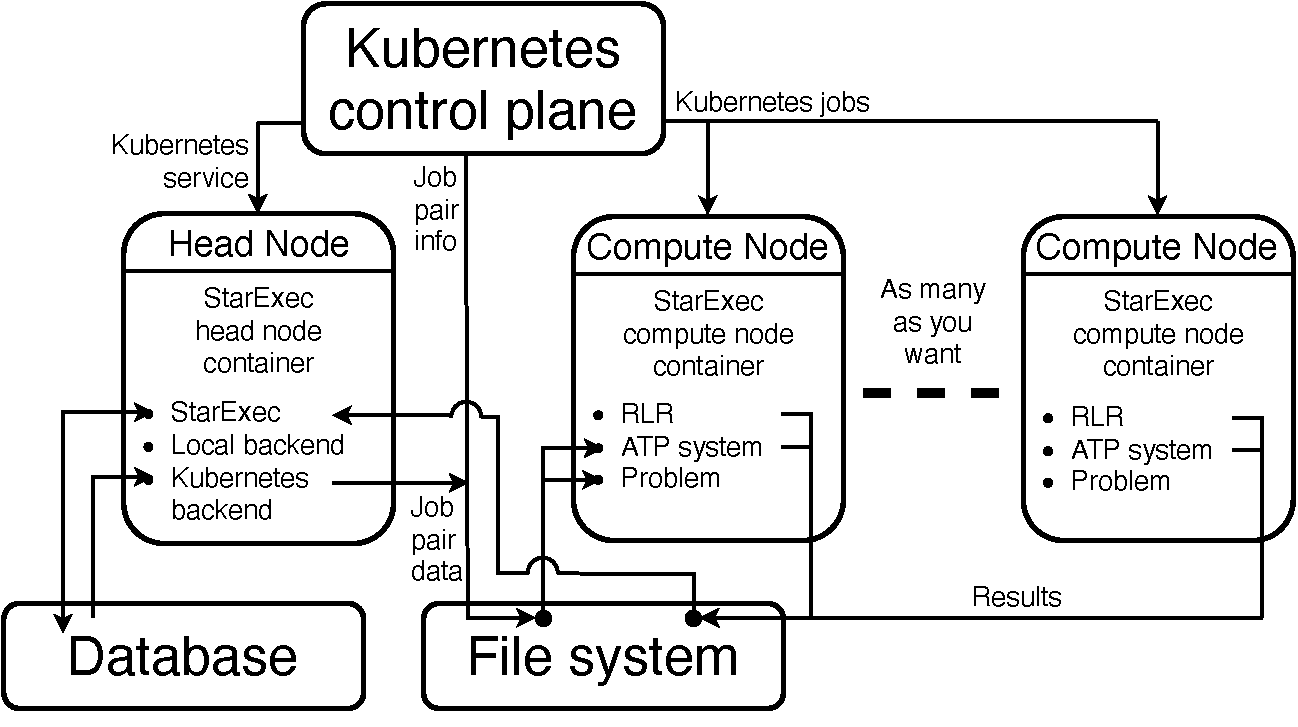
\includegraphics[width=0.8\textwidth]{ArchitectureK}
\caption{Projected StarExec generic architecture}
\label{ArchitectureK}
\end{center}
\end{figure}

\subsection{StarExec in AWS}

An Amazon Research Award\footnote{%
\href{https://www.amazon.science/research-awards/recipients/geoffrey-sutcliffe}
{Amazon Research Award, Fall 2023}.
Any opinions, findings, and conclusions or recommendations expressed in this material are those 
of the authors, and do not reflect the views of Amazon.} 
has been granted to deploy StarExec in AWS.
This will not only help fund the development efforts discussed in Section~\ref{FutureStarExec}, 
but will also fund a first fully-functional reference deployment of StarExec in the AWS cloud. 
The generic architecture in Figure~\ref{ArchitectureK} can, e.g., be instantiated using concrete 
AWS-managed services, as shown in Figure~\ref{ArchitectureAWS}.

\begin{figure}[htb]
\begin{center}
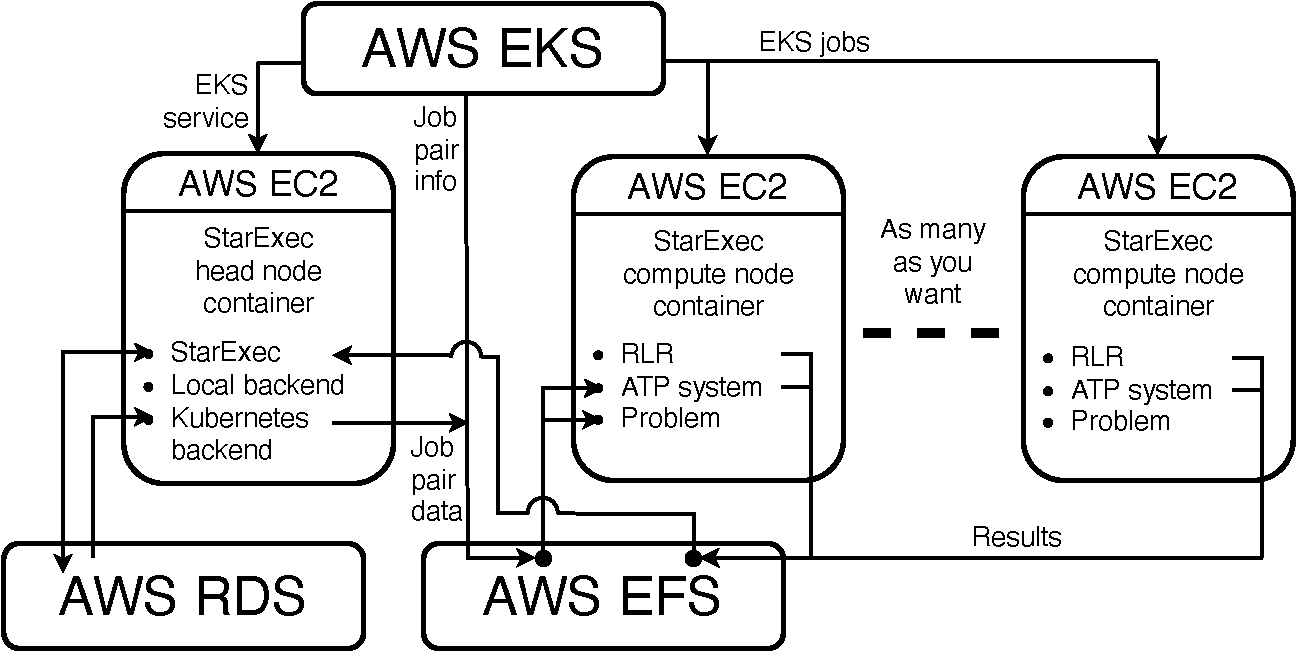
\includegraphics[width=0.8\textwidth]{ArchitectureAWS}
\caption{Architecture in AWS}
\label{ArchitectureAWS}
\end{center}
\end{figure}
\begin{packed_itemize}
	
\item The Kubernetes control plane can be managed by AWS Elastic Kubernetes Service (EKS).
\item The StarExec head and compute nodes can run on suitable Amazon EC2 instances, e.g., {\tt x2iedn.xlarge} which have four Intel Xeon Scalable vCPUs running up to 3.5GHz, and 128 GiB memory.
\item The database can be Amazon Relational Database (RDS).
\item The file system can be Amazon Elastic File System (EFS).
\item The ATP systems' containerisation can be made compatible with (possibly be exactly) the 
      Amazon Trusted Solver (ATS) format.\footnote{%
      As was recently used in the SMT and SAT competitions -- see \\
      \href{https://github.com/aws-samples/aws-batch-comp-infrastructure-sample}
      {\tt github.com/aws-samples/aws-batch-comp-infrastructure-sample}}
% \dav{@Geoff: do you have any refs for this "ATS format"? (it has an acronym so I assumed it 
% must be good documented on the web (apparently is not))}.
% Geoff: I heard about it when I had a meeting with the AWS people (Giles, Mike Whalen, etc).
\end{packed_itemize}

Leveraging AWS-managed services %introduces a degree of vendor lock-in, a situation that
will expedite the delivery of StarExec's initial cloud-native version to the community. 
This approach will particularly benefit teams planning to deploy StarExec on their own AWS 
accounts or through AWS grants.
% However, we maintain a strong commitment to open source and vendor neutrality, favoring 
% CNCF-endorsed projects and adhering strictly to the infrastructure-as-code paradigm for 
% StarExec's deployment into AWS. 
% This commitment is designed to ease the process for other teams, enabling them to effectively 
% bridge the ``last mile'' when deploying StarExec to non-managed AWS infrastructure or alternative 
% cloud providers, including private clouds and on-premise clusters.
The initial release will be rigorously tested through the migration of the TPTP community from 
StarExec Miami to the new StarExec AWS platform. 
We are particularly enthusiastic about collaborating with teams interested in deploying StarExec 
on their on-premise infrastructure or within university HPC clusters.

%--------------------------------------------------------------------------------------------------
\section{Conclusion}
\label{Conclusion}

This paper has described work being done to containerise StarExec and ATP systems so that they 
can be run on a broad range of computer platforms.
Additionally, this work explains plans to build backend in StarExec so that Kubernetes can be 
used to orchestration distribute of StarExec job pairs over whatever compute nodes are available.

This is ongoing work -- some of the work is still in progress, particularly embedding StarExec in 
Kubernetes on AWS.
Hopefully the future will include StarExec being flexibly available in online compute clusters.

%--------------------------------------------------------------------------------------------------
\bibliographystyle{plain}
\bibliography{Bibliography.bib}
%--------------------------------------------------------------------------------------------------
\appendix

\newpage
\section{E's {\tt run\_system} script}
\label{E_run_system}
{\small
\begin{verbatim}
#--------------------------------------------------------------------------------
#!/bin/tcsh

setenv HERE `dirname $0`
setenv TEMPDIR `mktemp -d`
setenv PROBLEMFILE $TEMPDIR/E---3.1_$$.p
onintr cleanup

#----Add extra ()s for THF and TXF
$HERE/tptp4X -t uniquenames4 -x $RLR_INPUT_FILE > $PROBLEMFILE

set SPCLine=`grep -E "^% SPC " $PROBLEMFILE`
if ("$SPCLine" != "") then
    set ProblemSPC = `expr "$SPCLine" : "^% SPC  *: *\([^ ]*\)"`
else
    set ProblemSPC = `$HERE/SPCForProblem $RLR_INPUT_FILE`
endif
set Mode = $RLR_INTENT

set CommonParameters="--delete-bad-limit=2000000000 --definitional-cnf=24 \
-s --print-statistics -R --print-version --proof-object --cpu-limit=$RLR_WC_LIMIT"
if ("$Mode" == "THM") then
    if (`expr "$ProblemSPC" : "TH0_.*"`) then
        echo "Running higher-order theorem proving"
        $HERE/eprover-ho $CommonParameters --auto-schedule=8 $PROBLEMFILE
    else
        echo "Running first-order theorem proving"
        $HERE/eprover $CommonParameters --auto-schedule=8 $PROBLEMFILE
    endif
else 
    echo "Running first-order model finding"
    $HERE/eprover $CommonParameters --satauto-schedule=8 $PROBLEMFILE
endif

cleanup:
    echo "% E exiting"
    rm -rf $TEMPDIR
#--------------------------------------------------------------------------------
\end{verbatim}
}

\newpage
\section{{\tt run\_image.py}}
\label{run_image}
{\small
\begin{verbatim}
#--------------------------------------------------------------------------------
#!/usr/bin/env python3

import argparse
import subprocess
import os, sys
import shutil

def getRLRArgs(args):
    mem_part = f" -M {args.memory_limit}" if args.memory_limit > 0 else ""
    return "--timestamp --watcher-data /dev/null -C " + \
f"{args.cpu_limit} -W {args.wall_clock_limit}{mem_part}"

def getEnvVars(args):
    return " ".join([f"-e {k}='{v}'" for k, v in [
        ("RLR_INPUT_FILE", "/artifacts/CWD/problemfile"),
        ("RLR_CPU_LIMIT", args.cpu_limit), ("RLR_WC_LIMIT", args.wall_clock_limit),
        ("RLR_MEM_LIMIT", args.memory_limit), ("RLR_INTENT", args.intent),
    ]])

def makeBenchmark(problem):
    if problem:
        shutil.copy(problem, "./problemfile")
    else:
        with open('./problemfile', 'w') as problemfile:
            problemfile.write(sys.stdin.read())

if __name__ == "__main__":
    parser = argparse.ArgumentParser("Wrapper for a podman call to a prover image")
    parser.add_argument("image_name", 
help="Image name, e.g., eprover:3.0.03-RLR-arm64")
    parser.add_argument("-P", "--problem",help="Problem file if not stdin")
    parser.add_argument("-C", "--cpu-limit", default=0, type=int, 
help="CPU time limit in seconds, default=none")
    parser.add_argument("-W", "--wall-clock-limit", default=0, type=int, 
help="Wall clock time limit in seconds, default=none")
    parser.add_argument("-M", "--memory-limit", default=0, type=int, 
help="Memory limit in MiB, default=none")
    parser.add_argument("-I", "--intent", default="THM", choices=["THM", "SAT"], 
help="Intention (THM, SAT, etc), default=THM")
    args = parser.parse_args()
    if args.wall_clock_limit == 0 and args.cpu_limit != 0:
        args.wall_clock_limit = args.cpu_limit

    command = f"podman run {getEnvVars(args)} -v .:/artifacts/CWD -t " + \
f"{args.image_name} {getRLRArgs(args)} run_system"
    makeBenchmark(args.problem)
    subprocess.run(command, shell=True)
    os.remove("./problemfile")
#--------------------------------------------------------------------------------
\end{verbatim}
}
%--------------------------------------------------------------------------------------------------
\end{document}
%--------------------------------------------------------------------------------------------------
